\section{Création d'une ligne de variations : \addbs{tkzTabVar}}
\subsection{Définition}

\begin{NewMacroBox}{tkzTabVar}{\oarg{local options}\var{el($1$),\dots,el($n$)}}
  avec \tkzname{el($i$) = s($i$) / e($i$)} ou bien     \tkzname{el($i$) = s($i$) / eg($i$) / ed($i$)}.
  
\noindent\tkzname{s($i$)} est une série de symboles à choisir dans le tableau ci-dessous. \tkzname{eg($i$)} et \tkzname{ed($i$)} sont des expressions mathématiques qui se placent à gauche et à droite des filets verticaux. \tkzname{e($i$)} est une expression centrée sur un filet.

\medskip  
 \begin{tabular}{llrl}
\toprule 
 Groupe 1& \emph{avec un seul signe} &&\\
\midrule 
\tkzname{s($i$)}  & Position des expressions & \tkzname{el($i$)}  &      \\
\midrule                                                                                   
\IargName{tkzTabVar}{$-~~~$}& expression  unique et centrée en bas  eg=ed   &  $-   $&$/e    $    \\
\IargName{tkzTabVar}{$+~~~$}& expression  unique et centrée en haut eg=ed   &  $+   $&$/e    $    \\
\IargName{tkzTabVar}{$~R~~$}& rien, on passe à l'expression  suivante           &  $~R  $&$(/)   $    \\
\IargName{tkzTabVar}{$-C$}  & prolongement par continuité en bas, centrée &  $-C  $&$/e    $    \\
\IargName{tkzTabVar}{$+C$}  & prolongement par continuité en haut, centrée&  $+C  $&$/e    $    \\
\IargName{tkzTabVar}{$-H$}  & expression en bas et centrée puis zone interdite  &  $-H  $&$/e    $    \\
\IargName{tkzTabVar}{$+H$}  & expression en haut et centrée puis zone interdite &  $+H  $&$/e    $    \\
\IargName{tkzTabVar}{$+D~~$}& discontinuité, expression en haut à gauche        &  $+D  $&$/e    $    \\
\IargName{tkzTabVar}{$-D~~$}& discontinuité, expression en bas à gauche         &  $-D  $&$/e    $    \\
\IargName{tkzTabVar}{$~D+~$}& discontinuité, expression en haut et à droite     &  $D+  $&$/e    $    \\
\IargName{tkzTabVar}{$~D-~$}& discontinuité, expression en bas et droite        &  $D-  $&$/e    $    \\
\IargName{tkzTabVar}{$+DH$} & discontinuité à gauche et en haut puis zone interdite&  $+DH $&$/e    $  \\
\IargName{tkzTabVar}{$-DH$} & discontinuité à gauche et en bas puis zone interdite &  $-DH $&$/e    $    \\
\IargName{tkzTabVar}{$+CH$} & prolongement par continuité puis zone interdite    &  $+CH $&$/e    $    \\
\IargName{tkzTabVar}{$-CH$} & idem mais  expression en bas et à gauche           &  $-CH $&$/e    $    \\
\midrule
 Groupe 2& \emph{avec deux signes}& &\\
\midrule 
\IargName{tkzTabVar}{$+D-$} & discontinuité,\hfill deux expressions    &  $+D- $&$/eg/ed$    \\
\IargName{tkzTabVar}{$-D+$} & discontinuité, \dots \hfill      qui sont    &  $-D+ $&$/eg/ed$    \\
\IargName{tkzTabVar}{$+D+$} & discontinuité, \dots \hfill soit  à gauche ,soit à droite &$+D+ $&$/eg/ed$    \\
\IargName{tkzTabVar}{$-D-$} & discontinuité, \dots \hfill soit en haut, soit en bas&$-D- $&$/eg/ed$    \\
\IargName{tkzTabVar}{$+CD+$}& prolongement par continuité à gauche et          &  $+CD+$&$/eg/ed$    \\
\IargName{tkzTabVar}{$-CD-$}& \dots \hfill  deux expressions qui sont        &  $-CD-$&$/eg/ed$    \\
\IargName{tkzTabVar}{$+CD-$}& \dots \hfill  soit  à gauche ,soit à droite  &  $+CD-$&$/eg/ed$    \\
\IargName{tkzTabVar}{$-CD+$}& \dots \hfill   soit en haut, soit en bas   &  $-CD+$&$/eg/ed$    \\
\IargName{tkzTabVar}{$+DC+$}& prolongement par continuité à droite et           &  $+DC+$&$/eg/ed$    \\
\IargName{tkzTabVar}{$-DC-$}& \dots \hfill  deux expressions qui sont          &  $-DC-$&$/eg/ed$    \\
\IargName{tkzTabVar}{$+DC-$}& \dots \hfill  soit  à gauche ,soit à droite      &  $+DC-$&$/eg/ed$    \\
\IargName{tkzTabVar}{$-DC+$}& \dots \hfill   soit en haut, soit en bas         &  $-DC+$&$/eg/ed$    \\
\IargName{tkzTabVar}{$+V+$} & comme une discontinuité mais sans double barre  et&  $+V+ $&$/eg/ed$    \\
\IargName{tkzTabVar}{$-V-$} & \dots \hfill  deux expressions qui sont     &  $-V- $&$/eg/ed$    \\
\IargName{tkzTabVar}{$+V-$} & \dots \hfill  soit  à gauche ,soit à droite &  $+V- $&$/eg/ed$    \\
\IargName{tkzTabVar}{$-V+$} & \dots \hfill   soit en haut, soit en bas    &  $-V+ $&$/eg/ed$    \\
\midrule
\tkzname{\textvisiblespace} & laisse la place vide dans certains cas& &   \\ 
\bottomrule
\end{tabular}

\medskip
\noindent\emph{La macro \tkzcname{tkzTabVar} nécessite un argument qui est une liste. Cette liste contient \tkzname{$n$} éléments correspondant aux \tkzname{$n$} antécédents de la première ligne. Chaque élément donne la position d'une ou de deux expressions par rapport à la ligne avec un signe $+$ (en haut) ou bien un signe $-$ (en  bas). Ces expressions sont, soit des images, soit des limites.}       

\noindent\emph{Les éléments \tkzname{el($i$)} ont pour forme~:\\
 soit \mbox{\tkzname{\{ s($i$)/ e($i$)\}}} ou bien \mbox{\tkzname{\{ s($i$)/ e($i$) / \}}}, soit \mbox{\tkzname{\{ s($i$)/ eg($i$) / ed($i$)\}}}.}
 
\noindent\emph{La première forme correspond aux symboles qui ne possèdent qu'un signe \tkzname{$+$} ou \tkzname{$-$} et qui  placent une seule expression; la seconde correspond aux symboles qui  possèdent deux signes et qui placent deux expressions. Les expressions sont des valeurs prises à gauche \tkzname{ eg($i$)\}} ou bien à droite \tkzname{ed($i$)} par la fonction ou encore des limites mais les expressions peuvent être vides. Un signe \tkzname{$+$} ou  \tkzname{$-$} à gauche (resp. à droite) des symboles correspond à \tkzname{eg($i$)} (resp. à \tkzname{ed($i$)}).}

\medskip
\begin{tabular}{lllc}
\toprule
\texttt{options}               & \texttt{défaut} & \texttt{définition}              \\
\midrule
\IoptName{tkzTabVar}{color}  & |black|         & couleur des flèches                \\
\IoptName{tkzTabVar}{help}   &  affiche la structure d'une ligne de variations      \\ 
 \bottomrule
\end{tabular} 

\end{NewMacroBox}  
  
 \medskip
Un schéma étant parfois plus simple qu'un long discours \dots

 \begin{center}
\begin{tikzpicture}
\tkzTabInit[lgt=2,espcl=3]{$x$/1,$f'(x)$/1,$f(x)$/3}%
{$0$,$1$,$2$,$+\infty$}%
\tkzTabLine{t,-,d,-,z,+,}%
\tkzTabVar{}% 
\node[below =3pt]  (FN12) at (N12){};  
\node[below =3pt]  (FN22) at (N22){}; 
\node[below =3pt]  (FN32) at (N32){};
\node[below =3pt]  (FN42) at (N42){};

\node[above =3pt]  (FN13) at (N13){};
\node[above =3pt]  (FN23) at (N23){};
\node[above =3pt]  (FN33) at (N33){};
\node[above =3pt]  (FN43) at (N43){};

\node[below right=3pt]  (FRN12) at (N12){};
\node[below right=3pt]  (FRN22) at (N22){}; 
\node[below right=3pt]  (FRN32) at (N32){};
\node[below right=3pt]  (FRN42) at (N42){};

\node[above right=3pt]  (FRN13) at (N13){};
\node[above right=3pt]  (FRN23) at (N23){};
\node[above right=3pt]  (FRN33) at (N33){};

\node[below left=3pt]  (FLN22) at (N22){}; 
\node[below left=3pt]  (FLN32) at (N32){};
\node[below left=3pt]  (FLN42) at (N42){};

\node[above left=3pt]  (FLN13) at (N13){};
\node[above left=3pt]  (FLN23) at (N23){};
\node[above left=3pt]  (FLN33) at (N33){};
\node[above left=3pt]  (FLN43) at (N43){};

\draw[fill=red!50] (FN12) circle(2pt)  node[below=2pt,text=red!50] {\small e} node[left=1cm,red] {$+$};
\draw[fill=red!50] (FN22) circle(2pt);
\draw[fill=red!50] (FN32) circle(2pt);
\draw[fill=red!50] (FN42) circle(2pt);

\draw[fill=red!50] (FN13) circle(2pt)  node[left=1cm,red] {$-$};
\draw[fill=red!50] (FN23) circle(2pt);
\draw[fill=red!50] (FN33) circle(2pt) node[above=2pt,text=red!50] {\small e};
\draw[fill=red!50] (FN43) circle(2pt);

\draw[fill=blue!30] (FRN12) circle(2pt);
\draw[fill=blue!30] (FRN22) circle(2pt) node[below right=2pt,text=blue!30] {\small ed};
\draw[fill=blue!30] (FRN32) circle(2pt);
\draw[fill=blue!30] (FRN13) circle(2pt);
\draw[fill=blue!30] (FRN23) circle(2pt);
\draw[fill=blue!30] (FRN33) circle(2pt);

\draw[fill=green!50] (FLN22) circle(2pt);
\draw[fill=green!50] (FLN32) circle(2pt);
\draw[fill=green!50] (FLN42) circle(2pt) node[below left =2pt,text=green!50] {\small eg};
\draw[fill=green!50] (FLN23) circle(2pt) node[above left =2pt,text=green!50] {\small eg};
\draw[fill=green!50] (FLN33) circle(2pt);
\draw[fill=green!50] (FLN43) circle(2pt);
\end{tikzpicture}
\end{center}
                                                       
\medskip
Pour les besoins de certains tableaux , j'ai employé les macros suivantes~:

\begin{tkzexample}[code only]
	\newcommand*{\va}{\colorbox{red!50}    {$\scriptscriptstyle V_a$}}
	\newcommand*{\vb}{\colorbox{blue!50}   {$\scriptscriptstyle V_b$}}
	\newcommand*{\vbo}{\colorbox{blue!50}  {$\scriptscriptstyle V_{b1}$}}
	\newcommand*{\vbt}{\colorbox{yellow!50}{$\scriptscriptstyle V_{b2}$}}
	\newcommand*{\vc}{\colorbox{gray!50}   {$\scriptscriptstyle V_c$}} 
	\newcommand*{\vd}{\colorbox{magenta!50}{$\scriptscriptstyle V_d$}} 
	\newcommand*{\ve}{\colorbox{orange!50} {$\scriptscriptstyle V_e$}}
\end{tkzexample}

\medskip
 \begin{center}
\begin{tikzpicture}
\tkzTabInit[lgt=2,espcl=3]{$x$/1,$f'(x)$/1,$f(x)$/3}%
{$0$,$1$,$2$,$+\infty$}%
  \tkzTabLine{t,-,d,-,z,+,}%
	\tkzTabVar{+/\va , -D+/\vb/\vc,-/\vd, +D/\ve}%
\end{tikzpicture}
\end{center}

\begin{tkzexample}[code only]
	\begin{tikzpicture}
	\tkzTabInit[lgt=2,espcl=3]{$x$/1,$f'(x)$/1,$f(x)$/3}%
	{$0$,$1$,$2$,$+\infty$}%
\tkzTabLine{t,-,d,-,z,+,}%
	\tkzTabVar{+/\va , -D+/\vb/\vc,-/\vd, +D/\ve}%
\end{tikzpicture}
\end{tkzexample}  

Commentaires : Les signes $+$ et $-$ permettent de positionner une extrémité de la flèche en haut ou en bas de la ligne. Ensuite, en présence d'un seul signe, une seule expression est nécessaire. La position par rapport à la colonne est donnée par la position du signe par rapport aux autres symboles (voir \tkzname{$+D$}).  \tkzname{$-D+$} nécessite deux expressions. 

\subsection{Utilisation des symboles}

\medskip
\bgroup\parindent=0pt
\begin{minipage}{7cm} 
\begin{tkzexample}[code only]
 {+ /\va , -/\vb }
\end{tkzexample}
  \begin{tikzpicture}
  \tkzTabInit[lgt=1]{ /0.5,/2 }{ a , b }
  \tkzTabVar% 
  {+ /\va , -/\vb }  
  \end{tikzpicture}
\end{minipage}
\hfill 
\begin{minipage}{7cm}
\begin{tkzexample}[code only]
 {-/\va   ,   +/\vb}
\end{tkzexample}
  \begin{tikzpicture}
  \tkzTabInit[lgt=1]{ /0.5,/2 }{ a , b }
  \tkzTabVar% 
{-/\va   ,   +/\vb} 
  \end{tikzpicture}
\end{minipage}

\begin{minipage}{7cm} 
\begin{tkzexample}[code only]
 {+/\va   ,   +/\vb}
\end{tkzexample}
  \begin{tikzpicture}
  \tkzTabInit[lgt=1]{ /0.5,/2 }{ a , b }
  \tkzTabVar% 
{+/\va   ,   +/\vb}   
  \end{tikzpicture}
\end{minipage}
\hfill 
\begin{minipage}{7cm}
\begin{tkzexample}[code only]
 {-/\va   ,   -/\vb}
\end{tkzexample}
  \begin{tikzpicture}
  \tkzTabInit[lgt=1]{ /0.5,/2 }{ a , b }
  \tkzTabVar% 
{-/\va   ,   -/\vb}   
  \end{tikzpicture}
\end{minipage}

\begin{minipage}{7cm} 
\begin{tkzexample}[code only]
 {+/\va  , -C / \vb}
\end{tkzexample}
  \begin{tikzpicture}
  \tkzTabInit[lgt=1]{ /0.5,/2 }{ a , b }
  \tkzTabVar% 
{+/\va  , -C / \vb}  
  \end{tikzpicture}
\end{minipage}
\hfill 
\begin{minipage}{7cm}
\begin{tkzexample}[code only]
{-/\va  , +C / \vb }\end{tkzexample}
  \begin{tikzpicture}
  \tkzTabInit[lgt=1]{ /0.5,/2 }{ a , b }
  \tkzTabVar% 
{-/\va  , +C / \vb }   
  \end{tikzpicture}
\end{minipage}

\begin{minipage}{7cm}
\begin{tkzexample}[code only]
 {+C  / \va ,  -C / \vb}
\end{tkzexample}
\begin{tikzpicture}
  \tkzTabInit[lgt=1]{ /0.5,/2 }{ a , b }
   \tkzTabVar% 
 {+C  / \va ,  -C / \vb } 
\end{tikzpicture}
\end{minipage}  
\hfill 
\begin{minipage}{7cm}
\begin{tkzexample}[code only]
 {-C /\va  , +C /\vb}
\end{tkzexample}
\begin{tikzpicture}
  \tkzTabInit[lgt=1]{ /0.5,/2 }{ a , b }
     \tkzTabVar% 
 {-C /\va  , +C /\vb}  
\end{tikzpicture}
\end{minipage}  

\begin{minipage}{7cm} 
\begin{tkzexample}[code only]
 { D+  /\va  ,  -/\vb}
\end{tkzexample}
  \begin{tikzpicture}
  \tkzTabInit[lgt=1]{ /0.5,/2 }{ a , b }
  \tkzTabVar% 
 { D+  /\va  ,  -/\vb}  
  \end{tikzpicture}
\end{minipage}
\hfill 
\begin{minipage}{7cm}
\begin{tkzexample}[code only]
 { D-  /\va  ,  +/\vb} 
\end{tkzexample}
  \begin{tikzpicture}
  \tkzTabInit[lgt=1]{ /0.5,/2 }{ a , b }
  \tkzTabVar
  { D-  /\va  ,  +/\vb}  
  \end{tikzpicture}
\end{minipage}

\begin{minipage}{7cm} 
\begin{tkzexample}[code only]
 {+/\va  , -D / \vb} 
\end{tkzexample}
  \begin{tikzpicture}
  \tkzTabInit[lgt=1]{ /0.5,/2 }{ a , b }
  \tkzTabVar% 
{+/\va  , -D / \vb}  
  \end{tikzpicture}
\end{minipage}
\hfill 
\begin{minipage}{7cm}
\begin{tkzexample}[code only]
 {-/\va  , +D / \vb }
\end{tkzexample}
  \begin{tikzpicture}
  \tkzTabInit[lgt=1]{ /0.5,/2 }{ a , b }
  \tkzTabVar% 
{-/\va  , +D / \vb }   
  \end{tikzpicture}
\end{minipage}

\begin{minipage}{7cm}
\begin{tkzexample}[code only]
 {D+ / \va , -D / \vb }
\end{tkzexample}
\begin{tikzpicture}
  \tkzTabInit[lgt=1]{ /0.5,/2 }{ a , b }
   \tkzTabVar% 
 {D+  / \va ,  -D / \vb } 
\end{tikzpicture}
\end{minipage}  
\hfill 
\begin{minipage}{7cm}
\begin{tkzexample}[code only]
 {D- /\va , +D /\vb}
\end{tkzexample}
\begin{tikzpicture}
  \tkzTabInit[lgt=1]{ /0.5,/2 }{ a , b }
     \tkzTabVar% 
 {D- /\va  , +D /\vb}  
\end{tikzpicture}
\end{minipage}  

\begin{minipage}{7cm}
\begin{tkzexample}[code only]
 {+/ \va , -/ \vb , +/ \vc}
\end{tkzexample}
\begin{tikzpicture}
\tkzTabInit[lgt=1,espcl=2.5]{ /0.5,/2 }{ a , b , c }
\tkzTabVar  {+/ \va , -/  \vb ,+/  \vc} 
\end{tikzpicture}
\end{minipage}   
\hfill 
\begin{minipage}{7cm}
\begin{tkzexample}[code only]
 {+/ \va ,-C/ \vb , +/  \vc/ }
\end{tkzexample}
\begin{tikzpicture}
\tkzTabInit[lgt=1,espcl=2.5]{ /0.5,/2 }{ a , b , c }
\tkzTabVar {+/ \va  ,-C/ \vb , +/  \vc/ } 
\end{tikzpicture}
\end{minipage} 

\begin{minipage}{7cm}
\begin{tkzexample}[code only]
 {-  /\va , R , +/\vc}
\end{tkzexample}
\begin{tikzpicture}
\tkzTabInit[lgt=1,espcl=2.5]{ /0.5,/2 }{ a , b , c }
\tkzTabVar% 
{-  /\va  ,  R,  +/\vc}     
\end{tikzpicture}
\end{minipage}   
\hfill 
\begin{minipage}{7cm}
\begin{tkzexample}[code only]
 {-  /\va , R , +/\vc}
\end{tkzexample}
\begin{tikzpicture}
\tkzTabInit[lgt=1,espcl=2.5]{ /0.5,/2}{ a , b , c }
\tkzTabVar% 
{-  /\va  ,  R  ,  +/\vc}  
\end{tikzpicture}
\end{minipage} 

\begin{minipage}{7cm}
\begin{tkzexample}[code only]
 {D-/\va , +DH/\vbo/ , }
\end{tkzexample}
\begin{tikzpicture}
\tkzTabInit[lgt=1,espcl=2.5]{ /0.5,/2 }{ a , b , c }
\tkzTabVar% 
{D-/\va  ,  +DH/\vbo/ ,  }     
\end{tikzpicture}
\end{minipage}   
\hfill 
\begin{minipage}{7cm}
\begin{tkzexample}[code only]
 {D-/\va  , -DH/\va/\vb ,  D+/}
\end{tkzexample}
\begin{tikzpicture}
\tkzTabInit[lgt=1,espcl=2.5]{ /0.5,/2 }{ a , b , c }
\tkzTabVar% 
{D-/\va  ,  -DH/\vbo ,  D+/}  
\end{tikzpicture}
\end{minipage} 

\begin{minipage}{7cm}
\begin{tkzexample}[code only]
 {D-/\va , +D-/\vbo/\vbt , +D/\vc}
\end{tkzexample}
\begin{tikzpicture}
\tkzTabInit[lgt=1,espcl=2.5]{ /0.5,/2 }{ a , b , c }
\tkzTabVar% 
{D-/\va  ,  +D-/\vbo/\vbt , +D/\vc}     
\end{tikzpicture}
\end{minipage}   
\hfill 
\begin{minipage}{7cm}
\begin{tkzexample}[code only]
 {D-/\va , +D-/\vbo/\vbt , +D/\vc}
\end{tkzexample}
\begin{tikzpicture}
\tkzTabInit[lgt=1,espcl=2.5]{ /0.5,/2 }{ a , b , c }
\tkzTabVar% 
{D-/\va  ,  -D-/\vbo/\vbt , +D/\vc}  
\end{tikzpicture}
\end{minipage} 

\begin{minipage}{7cm}
\begin{tkzexample}[code only]
 {+/\va , -D- / \vbo/\vbt , +/\vc}
\end{tkzexample}
\begin{tikzpicture}
\tkzTabInit[lgt=1,espcl=2.5]{ /0.5,/2 }{ a , b , c }
\tkzTabVar  {+/ \va , -D- /\vbo/\vbt,+/\vc  } 
\end{tikzpicture}
\end{minipage} 
\hfill 
\begin{minipage}{7cm}
\begin{tkzexample}[code only]
 {+ /\va,-DC- /\vbo/\vbt,+ /\vc}
\end{tkzexample}
\begin{tikzpicture}\tikzset{low/.style   = {above  =  15pt}}
\tkzTabInit[lgt=1,espcl=2.5]{ /0.5,/2 }{ a , b , c }
\tkzTabVar {+   /\va ,-DC- /\vbo/\vbt  ,+ /\vc} 
\end{tikzpicture}
\end{minipage}  

\begin{minipage}{7cm}
\begin{tkzexample}[code only]
 {D-/\va, +DC-/\vbo/\vbt, +D/\vc}
\end{tkzexample} 
\begin{tikzpicture}
\tkzTabInit[lgt=1,espcl=2.5]{ /0.5,/2 }{ a , b , c }
\tkzTabVar% 
{D-/\va  ,  +DC-/\vbo/\vbt ,+D/\vc} 
\end{tikzpicture}
\end{minipage}
\hfill 
\begin{minipage}{7cm}
\begin{tkzexample}[code only]
 {D+/\va , +DC-/\vbo/\vbt , +D/\vc}
\end{tkzexample}
\begin{tikzpicture}
\tkzTabInit[lgt=1,espcl=2.5]{ /0.5,/2 }{ a , b , c }
\tkzTabVar% 
{D+/\va  ,  +DC-/\vbo/\vbt ,+D/\vc}  
\end{tikzpicture}
\end{minipage}

\begin{minipage}{7cm}
\begin{tkzexample}[code only]
 {D-/\va , +CD-/\vbo/\vbt , +D/\vc}
\end{tkzexample}
\begin{tikzpicture}
\tkzTabInit[lgt=1,espcl=2.5]{ /0.5,/2 }{ a , b , c }
\tkzTabVar% 
{D-/\va  ,  +CD-/\vbo/\vbt , +D/\vc} 
\end{tikzpicture}
\end{minipage}
\hfill 
\begin{minipage}{7cm}
\begin{tkzexample}[code only]
 {D-/\va , +CD-/\vbo/\vbt ,+D/\vc}
\end{tkzexample}
\begin{tikzpicture}
\tkzTabInit[lgt=1,espcl=2.5]{ /0.5,/2 }{ a , b , c }
\tkzTabVar% 
{D+/\va , +CD-/\vbo/\vbt ,  +D/\vc}  
\end{tikzpicture}
\end{minipage}

\begin{minipage}{7cm}
\begin{tkzexample}[code only]
 {+/\va, -DC+ /\vbo/\vbt, - /\vc}
\end{tkzexample}
\begin{tikzpicture}
\tkzTabInit[lgt=1,espcl=2.5]{ /0.5,/2 }{ a , b , c }
\tkzTabVar  {+ /\va ,-DC+ /\vbo/\vbt , -/\vc} 
\end{tikzpicture}
\end{minipage} 
\hfill 
\begin{minipage}{7cm}
\begin{tkzexample}[code only]
 {D- /\va, -DC- /\vbo/\vbt,+D/\vc}
\end{tkzexample}
\begin{tikzpicture}\tikzset{low/.style           = {above       =  15pt}}
\tkzTabInit[lgt=1,espcl=2.5]{ /0.5,/2 }{ a , b , c }
\tkzTabVar% 
{D- /\va  , -DC- /\vbo/\vbt , +D/\vc}   
\end{tikzpicture}
\end{minipage}

\begin{minipage}{7cm}
\begin{tkzexample}[code only]
 {+/\va  , -CH /\vbo/\vbt , D+/}
\end{tkzexample}
\begin{tikzpicture}
\tkzTabInit[lgt=1,espcl=2.5]{ /0.5,/2 }{ a , b , c }
\tkzTabVar% 
{+/\va  , -CH /\vbo/\vbt , D+/}  
\end{tikzpicture}
\end{minipage}
\hfill
\begin{minipage}{7cm}
\begin{tkzexample}[code only]
 {+  /\va  , -CH/\vb,  //}
\end{tkzexample}
\begin{tikzpicture}
\tkzTabInit[lgt=1,espcl=2.5]{ /0.5,/2 }{ a , b , c }
\tkzTabVar% 
{+  /\va  , -CH/\vb,  //}  
\end{tikzpicture}
\end{minipage}

\begin{minipage}{7cm}
\begin{tkzexample}[code only]
 {+/\va , -V- /\vbo /\vbt, +/\vc}
\end{tkzexample}
\begin{tikzpicture}
\tkzTabInit[lgt=1,espcl=2.5]{ /0.5,/2 }{ a , b , c }
\tkzTabVar  {+/\va,-V- /\vbo /\vbt, +/\vc} 
\end{tikzpicture}
\end{minipage} 
\hfill 
\begin{minipage}{7cm}
\begin{tkzexample}[code only]
 {+/ \va ,-V+ / \vbo/ \vbt ,-/ \vc}
\end{tkzexample}
\begin{tikzpicture}
\tkzTabInit[lgt=1,espcl=2.5]{ /0.5,/2 }{ a , b , c }
\tkzTabVar  {+/ \va ,-V+ / \vbo/ \vbt ,-/ \vc}   
\end{tikzpicture}
\end{minipage} 

\begin{minipage}{7cm}
\begin{tkzexample}[code only]
 {+/ \va ,+V- /\vbo/ \vbt , -/\vc}
\end{tkzexample}
\begin{tikzpicture}
\tkzTabInit[lgt=1,espcl=2.5]{ /0.5,/2 }{ a , b , c }
\tkzTabVar  {+/ \va ,+V- / \vbo/ \vbt , -/\vc} 
\end{tikzpicture}
\end{minipage}   
\hfill 
\begin{minipage}{7cm}
\begin{tkzexample}[code only]
 {-/ \va, +V+ / \vbo/\vbt, -/\vc}
\end{tkzexample}
\begin{tikzpicture}
\tkzTabInit[lgt=1,espcl=2.5]{ /0.5,/2 }{ a , b , c }
\tkzTabVar  {-/ \va ,+V+ / \vbo / \vbt, -/\vc}   
\end{tikzpicture}
\end{minipage} 

\begin{minipage}{16cm}
\begin{tkzexample}[code only]
 {-/ \va ,+H/\vb,-/\vc, +/ \vd}
\end{tkzexample}
\begin{tikzpicture}
\tkzTabInit[lgt=1,espcl=3]{ /0.5,/2 }{ a , b , c , d }
\tkzTabVar  {-/  \va  ,+H/\vb,-/\vc, +/  \vd}   
\end{tikzpicture}
\end{minipage}

\begin{minipage}{16cm}
\begin{tkzexample}[code only]
 {+/  \va  ,-H/\vb,-/\vc, +/  \vd}
\end{tkzexample}
\begin{tikzpicture}
\tkzTabInit[lgt=1,espcl=3]{ /0.5,/2 }{ a , b , c , d }
\tkzTabVar  {+/  \va  ,-H/\vb,-/\vc, +/  \vd}   
\end{tikzpicture}
\end{minipage}

\begin{minipage}{16cm}
\begin{tkzexample}[code only]
 {-/  \va  , R , R , R , +/  \ve}
\end{tkzexample}
\begin{tikzpicture}
\tkzTabInit[lgt=1,espcl=3]{ /0.5,/2 }{ a , b , c , d , e}
\tkzTabVar  {-/  \va  ,R,R,R, +/  \ve}   
\end{tikzpicture}
\end{minipage}

\begin{minipage}{16cm}
\begin{tkzexample}[code only]
  {-/ \va , +/\vb , -DH/\vc , -/\vd , +/ \ve}
 \end{tkzexample}
\begin{tikzpicture}
\tkzTabInit[lgt=1,espcl=3]{ /0.5,/2 }{ a , b , c , d , e}
\tkzTabVar  {-/ \va  ,+/\vb ,-DH/\vc,-/\vd, +/ \ve}   
\end{tikzpicture}
\end{minipage} 

\begin{minipage}{16cm}
\begin{tkzexample}[code only]
 {D-/ \va , +DH/\vb/ , D-/\vc , +/\vd , +D/\ve}
\end{tkzexample}
\begin{tikzpicture}
\tkzTabInit[lgt=1,espcl=3]{ /0.5,/2 }{ a , b , c , d , e}
\tkzTabVar  {D-/  \va ,+DH/\vb/,D-/\vc,+/\vd, -D/\ve}   
\end{tikzpicture}
\end{minipage}
\egroup

\medskip
Commentaires
\begin{itemize}
  \item on peut employer la syntaxe suivante dans pratiquement tous les cas $s(i)/\ldots/\ldots$ mais alors il faut bien positionner les expressions;
  
  \item l'argument vide est employé parfois à la fin d'une ligne mais dans ce cas aucune flèche n'est tracée;
  
  \item $C+$ et $C-$ n'existent pas. $+C$ et $-C$ suffisent car les expressions sont centrées;
  \item  $D+$ et $D-$ existent .

\end{itemize}


\subsection{Utilisation des options}

\subsubsection{\texttt{\textcolor{red}{color}} : modification de la couleur des flèches}
Il est possible de personnaliser le tableau à l'aide de styles.
\begin{tkzexample}[vbox, small]
\begin{tikzpicture}
  \tkzTabInit[color,espcl=8]%
    {$x$   /1,%
     Signe\\ de $\dfrac{1}{x}$ /1.5,
     Variation\\ de $\ln$      /1.5}%
    {$0$,$+\infty$}%
  \tkzTabLine{d,+,}%
  \tkzTabVar[color=red]%
    {D-/    /  $-\infty$,+/  $+\infty$  /}
\end{tikzpicture}
\end{tkzexample} 
 
\subsubsection{\texttt{\textcolor{red}{help}} : affiche la structure du tableau} 
\Iopt{tkzTabVar}{help}   
Voir le chapitre personnalisation (\ref{pers})
\subsection{Utilisation des styles}
 
\subsubsection{Modification de la couleur d'une zone interdite}
\Istyle{tkzTabvar}{h style}
Si vous préférez hachurer une zone du tableau, alors  il faut modifier un style. 

Par défaut, \tkzname{h style}  est défini ainsi:
\begin{tkzexample}[code only] 
 \tikzset{h style/.style = {fill=gray,opacity=0.4}}
\end{tkzexample}

Une autre définition peut être :

\begin{tkzexample}[code only]
 \tikzset{h style/.style = {fill=red!50}}
\end{tkzexample}

\begin{tkzexample}[vbox,width=9cm]
\begin{tikzpicture}
 \tikzset{h style/.style = {fill=red!50}}
 \tkzTabInit[lgt=1,espcl=2]{$x$ /1,  $f$ /2}{$0$,$1$,$2$,$3$}%
 \tkzTabVar{+/ $1$  / , -CH/ $-2$ / , +C/  $5$, -/ $0$  /  }
\end{tikzpicture}
\end{tkzexample}  

\subsubsection{\texttt{\textcolor{red}{h style}} Zone interdite hachurée}
\Istyle{tkzTabVar}{h style}

\begin{tkzexample}[code only]
  \tikzset{h style/.style = {pattern=north west lines}} 
\end{tkzexample}
 Ce code permet d'hachurer la zone
 
\begin{tkzexample}[vbox,width=9cm,small]
\begin{tikzpicture}
 \tikzset{h style/.style = {pattern=north west lines}}
 \tkzTabInit[lgt=1,espcl=2]{$x$ /1,  $f$ /2}{$0$,$1$,$2$,$3$}%
 \tkzTabVar{+/ $1$  / , -CH/ $-2$ / , +C/  $5$, -/ $0$  /  }
\end{tikzpicture}
\end{tkzexample}


\subsubsection{\texttt{\textcolor{red}{arrow style}} style des flèches.}
\Istyle{tkzTabVar}{arrow} 
Le style des flèches est \tkzname{arrow style} et il est défini ainsi :

\begin{tkzexample}[code only]
   \tikzset{arrow style/.style   = {\cmdTAB@VA@color,
                                    ->,
                                    >           = latex',
                                    shorten >   =  2pt,
                                    shorten <   =  2pt}}
\end{tkzexample}

 On limite l'approche des nodes par les arrows. Voici une modification possible du style

\begin{tkzexample}[code only]
  \tikzset{arrow style/.style   = {blue,
                                   ->,
                                   >           = latex',
                                   shorten >   =  6pt,
                                   shorten <   =  6pt}}
\end{tkzexample}
 
 La couleur et l'approche des flèches sont modifiées.
 
\begin{tkzexample}[vbox,small]
\begin{tikzpicture}
  \tikzset{arrow style/.style   = {blue,
                                   ->,
                                   >           = latex',
                                   shorten >   =  6pt,
                                   shorten <   =  6pt}}  
  \tkzTabInit[espcl=5]{$x$ /1, $\ln x +1$ /1.5, $x \ln x$ /2}%
     {$0$ ,$1/\E$ , $+\infty$}%
  \tkzTabLine{d,-,z,+,}
  \tkzTabVar%
  { D+/   / $0$ ,%
     -/ \colorbox{black}{\textcolor{white}{$\dfrac{-1}{e}$}}/ ,%
     +/ $+\infty$  /  }%
\end{tikzpicture}
\end{tkzexample}

\subsubsection{\texttt{\textcolor{red}{node style}} Style des nodes}
\Istyle{tkzTabVar}{node style} 
Par défaut, Le style des nodes est \tkzname{node style} et il est défini ainsi : 
\begin{tkzexample}[code only]  
\tikzset{node style/.style    = {inner sep   =  2pt,
                                 outer sep   =  2pt,
                                 fill        =  \cmdTAB@tbs@colorT}}\end{tkzexample}
Si on veut apporter des modifications mais conserver une partie de ce style, on peut agir ainsi :

\begin{tkzexample}[code only]  
  \tikzset{node style/.append style = {draw,circle,fill=red!40,opacity=.4}}
\end{tkzexample}
 
 Par défaut les nodes sont des rectangles non tracés, ils deviennent des disques

\begin{tikzpicture}
  	\tikzset{node style/.append style    = {draw,circle,fill=red!40,opacity=.4}}
  \tkzTabInit[espcl=5]{$x$ /1, $\ln x +1$ /1.5, $x \ln x$ /2}%
     {$0$ ,$1/\E$ , $+\infty$}%
  \tkzTabLine{d,-,z,+,}
  \tkzTabVar%
  { D+/   / $0$ ,%
     -/ \colorbox{black}{\textcolor{white}{$\dfrac{-1}{e}$}}/ ,%
     +/ $+\infty$  /  }%
\end{tikzpicture}   
                               
\begin{tkzexample}[code only,small]
\begin{tikzpicture}
  	\tikzset{node style/.append style    = {draw,circle,fill=red!40,opacity=.4}}
  \tkzTabInit[espcl=5]{$x$ /1, $\ln x +1$ /1.5, $x \ln x$ /2}%
     {$0$ ,$1/\E$ , $+\infty$}%
  \tkzTabLine{d,-,z,+,}
  \tkzTabVar%
  { D+/   / $0$ ,%
     -/ \colorbox{black}{\textcolor{white}{$\dfrac{-1}{e}$}}/ ,%
     +/ $+\infty$  /  }%
\end{tikzpicture}
\end{tkzexample}  

\subsection{Quelques exemples}
\subsubsection{Fonction inverse}
Étude de la fonction inverse $i~:~ x \longmapsto \frac{1}{x}$ sur $]-\infty~;~0[ \cup ]0~;~+\infty[$ 


\begin{tkzexample}[vbox,small]
\begin{tikzpicture}
  \tkzTabInit[lgt=1.5,espcl=6.5]{$x$  /1,$i'(x)$  /1,$i$ /3}
                            {$-\infty$,$0$,$+\infty$}% 
  \tkzTabLine{,-,d,-,}
  \tkzTabVar{+/   $0$ /  ,-D+/ $-\infty$ / $+\infty$ , -/ $0$ /}
\end{tikzpicture}
\end{tkzexample}

\subsubsection{Fonction avec des paliers, emploi du symbole \texttt{\textcolor{red}{R}}}
Il est possible avec R de passer plusieurs valeurs.

\begin{tkzexample}[vbox,small]
\begin{tikzpicture}
 \tkzTabInit[espcl=4]{$x$  /1,$f'(x)$ /1,$f(x)$ /2}
                     {$0$ , $1$ ,$2$, $+\infty$}%
 \tkzTabLine         {d,+ , z,+ , z,+ ,        }
 \tkzTabVar{D-/ / $-\infty$,R/  /,R/   /,+/ $+\infty$   /}%
\end{tikzpicture}
\end{tkzexample}

\subsubsection{Zone interdite}

\begin{tkzexample}[vbox,small]
\begin{tikzpicture}
 \tkzTabInit[lgt=1,espcl=2]{$x$ /1,  $f$ /2}{$0$,$1$,$2$,$3$}%
 \tkzTabVar{+/ $1$ /   ,-DH/ $-\infty$ /   ,D+/   / $+\infty$, -/ $2$ / }
\end{tikzpicture}
\end{tkzexample}

\subsubsection{Zone interdite + prolongement par continuité}
\index{zone interdite}
\begin{tkzexample}[vbox,small]
\begin{tikzpicture}
 \tkzTabInit[lgt=1,espcl=2]{$x$ /1,  $f$ /2}{$0$,$1$,$2$,$3$}%
 \tkzTabVar{+/ $1$  / ,-CH/ $-2$ /, D+/ / $+\infty$,-/ $2$  / }
\end{tikzpicture}
\end{tkzexample}

\subsubsection{Zone interdite + double prolongement par continuité}
\index{prolongement par continuité} 
\begin{tkzexample}[vbox]
\begin{tikzpicture}
 \tkzTabInit[lgt=1,espcl=2]{$x$ /1,  $f$ /2}{$0$,$1$,$2$,$3$}%
 \tkzTabVar{+/ $1$  / , -CH/ $-2$ / , +C/  $5$, -/ $0$  /  }
\end{tikzpicture}
\end{tkzexample}

\subsubsection{Exemple d'une fonction partiellement constante}

Utilisation de l'option nocadre qui supprime le cadre extérieur, sinon on peut constater que l'on peut mettre pratiquement ce que l'on veut avec la macro \tkzcname{signe}.
\begin{tkzexample}[vbox,small]
\begin{tikzpicture}
 \tkzTab[nocadre,lgt=3,espcl=4]
  {$x$                  /1,
  Signe\\ de $f'(x)$    /1.5,
  Variations\\ de\\ $f$ /2}
  {$-\infty$, $-2$,$\dfrac{1}{\E}$,$\E$}%
  {z, <--- 0 --->,d, -, d, \genfrac{}{}{0pt}{0}{\text{signe de}}{ a}, d}
  {+/ $\dfrac{2}{3}$, +/ $\dfrac{2}{3}$,
   -D-/ $-\infty$ / $-\infty$,+D/ $+\infty$ }
\end{tikzpicture}
\end{tkzexample}

\subsubsection{Double variations}

\begin{tkzexample}[vbox,small]
\begin{tikzpicture}
 \tkzTabInit[espcl=6]
     {$x$   /1, $f''{x}$ /1,$f'(x)$ /2,  $f(x)$ /2}%
     {$0$ , $1$ , $+\infty$    }%
 \tkzTabLine{d,+,z,-, }%
 \tkzTabVar {D-/   /$1$,+/ $\E$ /,-/  $0$ /}%
 \tkzTabVar {D-/    /$-\infty$ ,R/    $0$   /, +/   $+8$ /}
\end{tikzpicture}
\end{tkzexample} 



\endinput